
\documentclass[11pt]{article}
\usepackage[a4paper,margin=1in]{geometry}
\usepackage{amsmath,amssymb}
\usepackage{graphicx}
\usepackage[dvipsnames]{xcolor}
\usepackage{hyperref}
\usepackage{enumitem}
\usepackage{tabularx}
\usepackage{longtable}
\usepackage{booktabs}
\usepackage[most]{tcolorbox}
\usepackage{titlesec}
\usepackage{xurl}
\usepackage{fancyhdr}
\usepackage{setspace}
\usepackage{tikz}
\usetikzlibrary{positioning,arrows.meta}
\usepackage[T1]{fontenc}
\usepackage{lmodern}
\setlength{\parindent}{0pt}
\setlength{\parskip}{8pt}
\setlength{\headheight}{14pt}
\setstretch{1.12}
\setlist[itemize]{leftmargin=1.5em, nosep}
\setlist[enumerate]{leftmargin=1.5em, nosep}
\providecommand{\tightlist}{\setlength{\itemsep}{0pt}\setlength{\parskip}{0pt}}
\hypersetup{colorlinks=true,linkcolor=MidnightBlue,urlcolor=MidnightBlue}
\pagestyle{fancy}
\fancyhf{}
\rhead{\thepage}
\renewcommand{\headrulewidth}{0pt}
\renewcommand{\footrulewidth}{0pt}
\titleformat{\section}{\Large\bfseries\color{MidnightBlue}}{\thesection}{0.6em}{}
\titleformat{\subsection}{\bfseries}{}{0em}{}


\begin{document}

\begin{center}\LARGE\bfseries Knowledge Representation for Agent Memory\end{center}

\begin{center}\large Block 3 Day 2\end{center}

\begin{tcolorbox}[colback=MidnightBlue!4,colframe=MidnightBlue,title={Session Overview},fonttitle=\bfseries,breakable]
\textbf{Session objective:} Move from informal descriptions to triples, IDs, structured memory, and controlled tool use.

\textbf{Timing target (min):} 71

\textbf{Topic anchors:} knowledge representation; triples; knowledge graph; internal knowledge; tool choice; planning

\textbf{Padlet board:} \url{https://padlet.com/qmul/b3-d2-1hyhngx342j150qn}
\end{tcolorbox}

\section*{Exercises}

\begin{tcolorbox}[colback=white,colframe=MidnightBlue,title={Q1 Starter Scenario},fonttitle=\bfseries,breakable]
\begin{center}
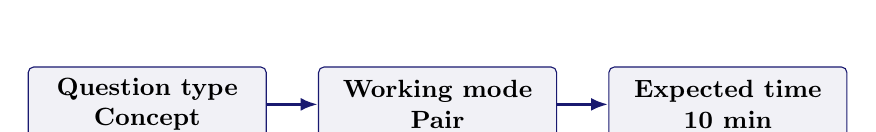
\begin{tikzpicture}[
node distance=0.65cm,
box/.style={draw=MidnightBlue, rounded corners=2pt, minimum height=0.95cm, align=center, font=\small\bfseries, fill=MidnightBlue!6, text width=0.23\linewidth},
arrow/.style={-{Latex[length=2.2mm]}, very thick, MidnightBlue}
]
\node[box] (type) {Question type\\Concept};
\node[box, right=of type] (mode) {Working mode\\Pair};
\node[box, right=of mode] (time) {Expected time\\10 min};
\draw[arrow] (type) -- (mode);
\draw[arrow] (mode) -- (time);
\end{tikzpicture}
\end{center}

{\large\bfseries\color{MidnightBlue} Prompt}\par\medskip
Imagine a robot that must make tea in your room. In the light of today's lecture, what would it need to know before acting, what would it need to check while acting, and what could still go wrong if the knowledge were badly represented?

{\large\bfseries\color{MidnightBlue} Task details}\par\medskip
\begin{itemize}\item \textbf{Type:} concept
\item \textbf{Mode:} pair
\item \textbf{Time:} 10 min
\item \textbf{Deliverable:} short scenario analysis
\item \textbf{Assessment focus:} explain what knowledge a robot needs before it can act reliably
\item \textbf{Expected length:} 3 knowledge items + 2 checks + 1 risk\end{itemize}

{\large\bfseries\color{MidnightBlue} How to submit}\par\medskip
Post one pair Padlet comment with three knowledge items, two runtime checks, and one likely failure.

{\large\bfseries\color{MidnightBlue} Discussion in class}\par\medskip
Which missing fact would break the task first?

{\large\bfseries\color{MidnightBlue} Why this helps}\par\medskip
Useful for short questions that ask why knowledge representation matters before planning or action.

{\large\bfseries\color{MidnightBlue} References}\par\medskip
\begin{itemize}\item Russell \& Norvig (2021) AIMA 4e, Ch.10, pp.314-343
\item Poole \& Mackworth (2023) 3e, Ch.16, pp.701-730\end{itemize}
\end{tcolorbox}

\begin{tcolorbox}[colback=white,colframe=MidnightBlue,title={Q2 Structured Problem},fonttitle=\bfseries,breakable]
\begin{center}
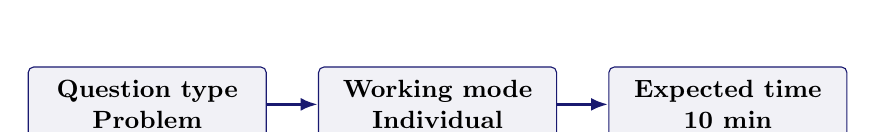
\begin{tikzpicture}[
node distance=0.65cm,
box/.style={draw=MidnightBlue, rounded corners=2pt, minimum height=0.95cm, align=center, font=\small\bfseries, fill=MidnightBlue!6, text width=0.23\linewidth},
arrow/.style={-{Latex[length=2.2mm]}, very thick, MidnightBlue}
]
\node[box] (type) {Question type\\Problem};
\node[box, right=of type] (mode) {Working mode\\Individual};
\node[box, right=of mode] (time) {Expected time\\10 min};
\draw[arrow] (type) -- (mode);
\draw[arrow] (mode) -- (time);
\end{tikzpicture}
\end{center}

{\large\bfseries\color{MidnightBlue} Prompt}\par\medskip
Describe how to make a cup of tea as a series of short facts rather than commands. Write eight facts that a robot could store and later reason over.

{\large\bfseries\color{MidnightBlue} Task details}\par\medskip
\begin{itemize}\item \textbf{Type:} problem
\item \textbf{Mode:} individual
\item \textbf{Time:} 10 min
\item \textbf{Deliverable:} fact list
\item \textbf{Assessment focus:} convert an action description into stored knowledge facts
\item \textbf{Expected length:} 8 short facts\end{itemize}

{\large\bfseries\color{MidnightBlue} How to submit}\par\medskip
Post your own Padlet comment as eight short facts, not instructions.

{\large\bfseries\color{MidnightBlue} Discussion in class}\par\medskip
Which of your facts describes a relation between two entities?

{\large\bfseries\color{MidnightBlue} Why this helps}\par\medskip
Direct practice for turning natural language into machine-usable facts.

{\large\bfseries\color{MidnightBlue} References}\par\medskip
\begin{itemize}\item Russell \& Norvig (2021) AIMA 4e, Ch.10, pp.314-343
\item Poole \& Mackworth (2023) 3e, Ch.16, pp.701-730\end{itemize}
\end{tcolorbox}

\begin{tcolorbox}[colback=white,colframe=MidnightBlue,title={Q3 Structured Problem},fonttitle=\bfseries,breakable]
\begin{center}
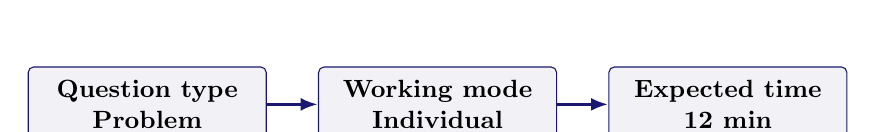
\begin{tikzpicture}[
node distance=0.65cm,
box/.style={draw=MidnightBlue, rounded corners=2pt, minimum height=0.95cm, align=center, font=\small\bfseries, fill=MidnightBlue!6, text width=0.23\linewidth},
arrow/.style={-{Latex[length=2.2mm]}, very thick, MidnightBlue}
]
\node[box] (type) {Question type\\Problem};
\node[box, right=of type] (mode) {Working mode\\Individual};
\node[box, right=of mode] (time) {Expected time\\12 min};
\draw[arrow] (type) -- (mode);
\draw[arrow] (mode) -- (time);
\end{tikzpicture}
\end{center}

{\large\bfseries\color{MidnightBlue} Prompt}\par\medskip
A campus-support assistant must answer: Who teaches EBU6505? Where is the office of Dr\_Riasat\_Islam? When are EBU6505 office hours? Write 6-8 triples using clear IDs such as Module\_EBU6505, Dr\_Riasat\_Islam, and TB\_3\_335.

{\large\bfseries\color{MidnightBlue} Task details}\par\medskip
\begin{itemize}\item \textbf{Type:} problem
\item \textbf{Mode:} individual
\item \textbf{Time:} 12 min
\item \textbf{Deliverable:} triple set with IDs
\item \textbf{Assessment focus:} write clear triples using stable identifiers and meaningful relations
\item \textbf{Expected length:} 6-8 triples + 1 ID note\end{itemize}

{\large\bfseries\color{MidnightBlue} How to submit}\par\medskip
Post your own Padlet comment with the triples and one short note explaining the IDs you chose.

{\large\bfseries\color{MidnightBlue} Discussion in class}\par\medskip
Why are stable IDs better than storing only surface strings?

{\large\bfseries\color{MidnightBlue} Why this helps}\par\medskip
Direct practice for converting a simple support scenario into triples with explicit identifiers.

{\large\bfseries\color{MidnightBlue} References}\par\medskip
\begin{itemize}\item Russell \& Norvig (2021) AIMA 4e, Ch.10, pp.314-343
\item Poole \& Mackworth (2023) 3e, Ch.16, pp.701-730\end{itemize}
\end{tcolorbox}

\begin{tcolorbox}[colback=white,colframe=MidnightBlue,title={Q4 Stretch Extension},fonttitle=\bfseries,breakable]
\begin{center}
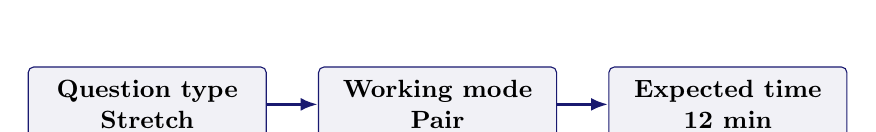
\begin{tikzpicture}[
node distance=0.65cm,
box/.style={draw=MidnightBlue, rounded corners=2pt, minimum height=0.95cm, align=center, font=\small\bfseries, fill=MidnightBlue!6, text width=0.23\linewidth},
arrow/.style={-{Latex[length=2.2mm]}, very thick, MidnightBlue}
]
\node[box] (type) {Question type\\Stretch};
\node[box, right=of type] (mode) {Working mode\\Pair};
\node[box, right=of mode] (time) {Expected time\\12 min};
\draw[arrow] (type) -- (mode);
\draw[arrow] (mode) -- (time);
\end{tikzpicture}
\end{center}

{\large\bfseries\color{MidnightBlue} Prompt}\par\medskip
A travel platform stores Hotel\_H888, the city Beijing, a star rating, a user review, and a price band. Represent this as triples and make clear which parts are entity links and which parts are attributes.

{\large\bfseries\color{MidnightBlue} Task details}\par\medskip
\begin{itemize}\item \textbf{Type:} stretch
\item \textbf{Mode:} pair
\item \textbf{Time:} 12 min
\item \textbf{Deliverable:} mini data model
\item \textbf{Assessment focus:} separate entities, attributes, and review facts in a realistic triple design
\item \textbf{Expected length:} 6 triples + 2 attribute notes\end{itemize}

{\large\bfseries\color{MidnightBlue} How to submit}\par\medskip
Post one pair Padlet comment with six triples and two short notes explaining attribute choices.

{\large\bfseries\color{MidnightBlue} Discussion in class}\par\medskip
Which information would you not model as a new entity?

{\large\bfseries\color{MidnightBlue} Why this helps}\par\medskip
Useful for questions about entity-versus-attribute choices and practical triple design.

{\large\bfseries\color{MidnightBlue} References}\par\medskip
\begin{itemize}\item Russell \& Norvig (2021) AIMA 4e, Ch.10, pp.314-343
\item Poole \& Mackworth (2023) 3e, Ch.16, pp.701-730\end{itemize}
\end{tcolorbox}

\begin{tcolorbox}[colback=white,colframe=MidnightBlue,title={Q5 Collaborative Mini-Case},fonttitle=\bfseries,breakable]
\begin{center}
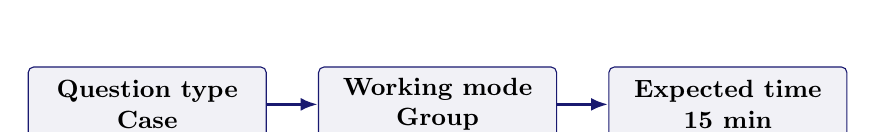
\begin{tikzpicture}[
node distance=0.65cm,
box/.style={draw=MidnightBlue, rounded corners=2pt, minimum height=0.95cm, align=center, font=\small\bfseries, fill=MidnightBlue!6, text width=0.23\linewidth},
arrow/.style={-{Latex[length=2.2mm]}, very thick, MidnightBlue}
]
\node[box] (type) {Question type\\Case};
\node[box, right=of type] (mode) {Working mode\\Group};
\node[box, right=of mode] (time) {Expected time\\15 min};
\draw[arrow] (type) -- (mode);
\draw[arrow] (mode) -- (time);
\end{tikzpicture}
\end{center}

{\large\bfseries\color{MidnightBlue} Prompt}\par\medskip
Design a small internal knowledge graph for a university assistant that answers timetable, office-hour, room-change, and contact questions. Include the node types, key relations, and a short retrieval flow.

{\large\bfseries\color{MidnightBlue} Task details}\par\medskip
\begin{itemize}\item \textbf{Type:} case
\item \textbf{Mode:} group
\item \textbf{Time:} 15 min
\item \textbf{Deliverable:} memory-graph design
\item \textbf{Assessment focus:} design a small internal knowledge graph for an assistant with reusable memory
\item \textbf{Expected length:} 4 node types + 5 relations + 3-step retrieval flow\end{itemize}

{\large\bfseries\color{MidnightBlue} How to submit}\par\medskip
Post one group Padlet comment with four node types, five relations, and a three-step retrieval flow.

{\large\bfseries\color{MidnightBlue} Discussion in class}\par\medskip
What is the smallest graph that would still make the assistant useful?

{\large\bfseries\color{MidnightBlue} Why this helps}\par\medskip
Supports case questions on internal memory, graph structure, and retrieval design.

{\large\bfseries\color{MidnightBlue} References}\par\medskip
\begin{itemize}\item Russell \& Norvig (2021) AIMA 4e, Ch.10, pp.314-343
\item Poole \& Mackworth (2023) 3e, Ch.16, pp.701-730\end{itemize}
\end{tcolorbox}

\begin{tcolorbox}[colback=white,colframe=MidnightBlue,title={Q6 Exam-Style Constructed Response},fonttitle=\bfseries,breakable]
\begin{center}
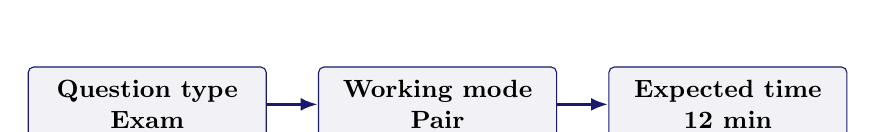
\begin{tikzpicture}[
node distance=0.65cm,
box/.style={draw=MidnightBlue, rounded corners=2pt, minimum height=0.95cm, align=center, font=\small\bfseries, fill=MidnightBlue!6, text width=0.23\linewidth},
arrow/.style={-{Latex[length=2.2mm]}, very thick, MidnightBlue}
]
\node[box] (type) {Question type\\Exam};
\node[box, right=of type] (mode) {Working mode\\Pair};
\node[box, right=of mode] (time) {Expected time\\12 min};
\draw[arrow] (type) -- (mode);
\draw[arrow] (mode) -- (time);
\end{tikzpicture}
\end{center}

{\large\bfseries\color{MidnightBlue} Prompt}\par\medskip
A university assistant can use timetable search, policy search, calculator, and email-draft tools. Explain how it should choose a tool and why planning should be separated from execution.

{\large\bfseries\color{MidnightBlue} Task details}\par\medskip
\begin{itemize}\item \textbf{Type:} exam
\item \textbf{Mode:} pair
\item \textbf{Time:} 12 min
\item \textbf{Deliverable:} structured explanation
\item \textbf{Assessment focus:} explain tool-choice reasoning and why planning should be separated from execution
\item \textbf{Expected length:} 180-240 words\end{itemize}

{\large\bfseries\color{MidnightBlue} How to submit}\par\medskip
Post one pair Padlet comment with a clear policy, one failure case, and one recovery step.

{\large\bfseries\color{MidnightBlue} Discussion in class}\par\medskip
What goes wrong if the assistant executes a tool before it has a plan?

{\large\bfseries\color{MidnightBlue} Why this helps}\par\medskip
Matches longer answers about reasoning policies, tool selection, and controlled execution.

{\large\bfseries\color{MidnightBlue} References}\par\medskip
\begin{itemize}\item Russell \& Norvig (2021) AIMA 4e, Ch.10, pp.314-343
\item Poole \& Mackworth (2023) 3e, Ch.16, pp.701-730
\item https://developers.google.com/search/docs/appearance/structured-data/intro-structured-data\end{itemize}
\end{tcolorbox}

\section*{Submission Instructions}

Use the seeded Padlet posts for Q1--Q6. Q2 and Q3 are individual. Q1, Q4, and Q6 are pair tasks. Q5 should be one joint group comment. Start each comment with your names or group label.

\section*{Whole-Class Debrief Prompts}

\begin{itemize}
\tightlist
\item
  Which change made the tea-making knowledge more machine-usable?
\item
  Which triple-design choice made the university assistant easier to query?
\item
  Where should planning stop and execution begin in a tool-using assistant?
\end{itemize}

\section*{Exam Transfer Note (Day-Level)}

Maps to exam questions on fact representation, triples, IDs, entities versus attributes, internal memory graphs, and tool-choice reasoning.

\end{document}
